\documentclass[ruledheader,noindentfirst,anapcustomindent,abntfigtabnum,tocpage=plain]{abnt}

\usepackage{amsmath, amssymb, amsthm, verbatim, amsfonts, amstext}
%\usepackage[latin1]{inputenc}
\usepackage[brazilian]{babel}
\usepackage[utf8]{inputenc}
\usepackage[T1]{fontenc}
\usepackage{dropping}
\usepackage{graphicx}
\usepackage[hang,small,bf]{caption}
\usepackage[abnt-etal-list=0,abnt-etal-text=it,abnt-and-type=&,abnt-emphasize=bf,abnt-full-initials=yes,alf,bibjustif]{abntcite}
\usepackage{fancyhdr}
\usepackage{makeidx}
\usepackage[none]{hyphenat}
\usepackage{color}
\usepackage{subfig}
\usepackage{algorithms}
\usepackage{algorithmic}
\usepackage{mdwlist}
\usepackage{bm}
\usepackage[titletoc,title]{appendix}
\usepackage{ltxtable}
\usepackage{longtable}
\usepackage{supertabular}
\usepackage{indentfirst}
\usepackage{color}
\usepackage{icomma}
\usepackage{url}

\usepackage{float}
\usepackage{multirow}
\usepackage{longtable}
\usepackage{enumerate}
\usepackage[table]{xcolor}
\usepackage{pifont}

\usepackage{pgfplots}

\sloppy

%
%Tradução do pacote Algorithm para portugues
%
\renewcommand{\algorithmicrequire}{\textbf{Entrada:}}
\renewcommand{\algorithmicensure}{\textbf{Saída:}}
\renewcommand{\algorithmicend}{\textbf{fim}}
\renewcommand{\algorithmicif}{\textbf{se}}
\renewcommand{\algorithmicthen}{\textbf{então}}
\renewcommand{\algorithmicelse}{\textbf{senão}}
\renewcommand{\algorithmicelsif}{\algorithmicelse \, \algorithmicif}
\renewcommand{\algorithmicendif}{\algorithmicend \, \algorithmicif}
\renewcommand{\algorithmicfor}{\textbf{para}}
\renewcommand{\algorithmicforall}{\textbf{para todo}}
\renewcommand{\algorithmicdo}{\textbf{fazer}}
\renewcommand{\algorithmicendfor}{\algorithmicend \, \algorithmicfor}
\renewcommand{\algorithmicwhile}{\textbf{enquanto}}
\renewcommand{\algorithmicendwhile}{\algorithmicend \, \algorithmicwhile}
\renewcommand{\algorithmicloop}{\textbf{laço}}
\renewcommand{\algorithmicendloop}{\algorithmicend \, \algorithmicloop}
\renewcommand{\algorithmicrepeat}{\textbf{repetir}}
\renewcommand{\algorithmicuntil}{\textbf{até}}
\renewcommand{\algorithmiccomment}[1]{\{#1\}}
\renewcommand{\listalgorithmname}{Lista de Algoritmos}
\floatname{algorithm}{Algoritmo}
%%%%%%%%%%%%%%%%%%%%%%%%%%%%%%%%%%%%%%%%%%%%%%%%%%%%%%%%%%%%%%%%%%%%%%%%%%%%%%%%%%%
\newcommand*\rot{\rotatebox{90}}
\newcommand*\V{\ding{51}}
\newcommand\tab[1][1cm]{\hspace*{#1}}

\makeindex

%%%% O arquivo estiloCAP.tex possui as definições para ciação do estilo de capítulo (fonte de título, barras horizontais, etc.)
% ele não gera texto de saída, é um arquivo de configuração somente
%
% %Estilo de formatação de capítulos

\makeatletter
\newcommand{\thechapterwords}
{ \ifcase \thechapter\or 1\or 2\or 3\or 4\or 5\or6\or 7\or 8\or 9\or 10\or 11\fi}

\def\@makechapterhead#1{%
\vspace*{10\p@}%
{\parindent \z@  \reset@font

\scshape \@chapapp{} \thechapterwords
\quad %
\par\nobreak
\vspace*{10\p@}%
\interlinepenalty\@M
\hrule
\vspace*{10\p@}%
\Huge \bfseries #1\par\nobreak
\par
\vspace*{10\p@}%
\hrule
\vskip 40\p@
}}
\def\@makeschapterhead#1{%
\vspace*{10\p@}%
{\parindent \z@ \centering \reset@font
\par\nobreak
\vspace*{10\p@}%
\interlinepenalty\@M
\hrule
\vspace*{10\p@}%
\Huge \bfseries #1\par\nobreak
\par
\vspace*{10\p@}%
\hrule
\vskip 40\p@
%\vskip 100\p@
}}
%%%%%%%%%%%%%%%%%%%%%%%%%%%%%%%%%%%%%%%%%%%%%%%FIM DO PREAMBULO%%%%%%%%%%%%%%%%%%%%%%%%%%%%%%%%%%%%%%%%%%%%%%%%%%%%%%%%%%%%%%%%%%





\begin{document}

%%%%% IMPORTANTE: ALTERA O TEXTO ENTRE ARIAL E TIMES NEW ROMAN (ALTERNAR OS COMENTÁRIOS)
%
%%%%%%%%%%%%%%%%%%%%%PARA UTILIZAR ARIAL%%%%%%%%%%%%%%%%%%%%%%%
%
\fontfamily{phv}                    %fonte Arial
\renewcommand{\rmdefault}{phv}      %
%
%%%%%%%%%%%%%%%%%%%%%PARA UTILIZAR TIMES%%%%%%%%%%%%%%%%%%%%%%%
%
%\fontfamily{ptm}               %fonte Times
%\renewcommand{\rmdefault}{ptm} %
%
%%%%%%%%%%%%%%%%%%%%%%%%%%%%%%%%%%%%%%%%%%%%%%%%%%%%%%%%%%%%%%%

%%%%%%%%%%%%%Arquivos .tex com os elementos pré-textuais
%
\thispagestyle{empty}

\vfill
 \begin{center}
    \begin{figure}[t]
     \centering
            % 
\includegraphics[width=5cm]{figures/logo.pdf}\\[-0.1in]
            
\includegraphics[width=15cm]{figuras/logo-uit.pdf}\\[-0.1in]
     \end{figure}

    {\large\bfseries UNIVERSIDADE DE ITAÚNA} \\
    {\large\bfseries PRÓ-REITORIA DE ENSINO} \\
    {\large\bfseries COORDENAÇÃO DE CIÊNCIA DA COMPUTACAO}  \\ 
    {\large\bfseries BACHARELADO EM CIÊNCIA DA COMPUTAÇÃO}  \\ 

    \vspace*{1in}
    \begin{large} \bfseries Eugênio Cunha\end{large}\\[0.4in]

    \vspace*{4cm}
    \noindent \\
    \large\bfseries{APRENDIZADO DE MÁQUINA APLICADO À VALORAÇÃO DAS COMPETÊNCIAS DE UMA REDAÇÃO} \\
    \vfill
    \large\bfseries{ ITAÚNA \\ 2017}
\end{center}

\normalsize
\begin{titlepage}
\vfill
\begin{center}

    {\large EUGÊNIO CUNHA\\}
    \vspace{2cm}
    {\Large \textsc{APRENDIZADO DE MÁQUINA APLICADO À VALORAÇÃO DE REDAÇÕES}\\}
    \vspace{1cm}
    \hspace{.45\linewidth}
    \begin{minipage}{.50\linewidth}

            Projeto submetido à Coordenadoria do Curso de Bacharelado 
            em Ciência da Computação da Universidade de Itaúna - Campus Verde, como requisito 
            parcial para obtenção do grau de Bacharel em Ciência da Computação.

            \vspace{0.5 cm}

            Área de pesquisa: Aprendizagem de Máquina

            \vspace{0.5 cm}

            Orientador: Prof. Dr. Marco Túlio Alves N Rodrigues
    
    \end{minipage}

    \vspace{2cm}
    \vfill
    {\large Itaúna\\ 2017}
\end{center}

\end{titlepage}
\begin{folhadeaprovacao}
\setlength{\ABNTsignthickness}{0.2pt}
\setlength{\ABNTsignskip}{1.7cm}

\begin{center}

\includegraphics[width=2.5cm]{figuras/brasao_uit.pdf}\\
            {UNIVERSIDADE DE ITAÚNA} \\
            {COORDENAÇÃO DE CIÊNCIA DA COMPUTAÇÃO}  \\

    \vspace{1.5cm}
                                    {EUGÊNIO CUNHA}\\
    \bfseries{}
\end{center}

Este projeto foi julgada adequada para a obten\c{c}\~{a}o do Grau de Bacharel em Ciência da Computação, sendo aprovada pela coordenação de ciência da computação do curso de Bacharelado em Ciência da Computação
do Campus verde da Universidade de Itaúna e pela banca examinadora:

    \vspace{0.15cm}
    \assinatura{Orientador: Prof. Dr. Marco Túlio Alves N Rodrigues\\ Universidade de Itaúna- UIT}
    \assinatura{Avaliador: Coord. Prof. Dr. Felipe Domingos da Cunha \\ Universidade de Itaúna- UIT}
    \vspace{0.15cm}%\vfill

    \begin{center}
        Itaúna, 19 de Junho de 2017
    \end{center}
\end{folhadeaprovacao}

\begin{flushright}
\begin{minipage}[r]{10cm}
\vspace{15cm}
\hfill Dedico este trabalho a Davi, meu filho, sempre preocupado em 
proporcionar um minuto de pausa para brincadeiras durante minhas horas de 
estudo, ``meus melhores minutos''! \\
% \begin{flushright}
% Albert Einstein
% \end{flushright}
\end{minipage}
\end{flushright}
\include{pre-textuais/agradecimentos}
%\thispagestyle{empty}


\begin{flushright}
\begin{minipage}[r]{10cm}
\vspace{18cm}
``Os computadores são incrivelmente rápidos, precisos e burros; os homens são incrivelmente lentos, imprecisos e brilhantes; juntos, seus poderes ultrapassam os limites da imaginação''.
\begin{flushright}
Albert Einstein
\end{flushright}
\end{minipage}
\end{flushright}
\pagestyle{plain}%%%%% Utilizar ESTILO PLAIN AQUI%%%%%%%
\chapter*{Resumo}

\noindent Este trabalho baseou-se na avaliação das competências exigidas em um 
texto de redação do tipo dissertativo-argumentativo com temas diversificados 
de ordem social, científica, cultural ou política. Fundamentou-se no estudo 
das técnicas de aprendizado de máquina supervisionado que provê uma gama 
diversificada de algoritmos poderosos para classificações de textos.

O objetivo deste trabalho é classificar as competências exigidas em um texto de 
redação a partir do treinamento de um modelo de aprendizado de máquina com
base em um \textit{corpus} de redações avaliadas seguindo as competências 
exigidas em uma redação do tipo dissertativa-argumentativa.

A compilação de um \textit{corpus} de redações para treinamento e teste de um 
modelo de aprendizado de máquina exigiu a prática de extração de informações 
que compreende técnicas e algoritmos que realisam duas tarefas importantes: a 
identificação de informações desejadas a partir de documentos estruturados e 
não-estruturados, e o armazenamento dessas informações em um formato apropriado 
para uso futuro. Afim de se avaliar a eficácia dos classificadores, 
vários experimentos foram executados usando-se um \textit{corpus} extraido do 
banco de redações da UOL ~\cite{uol_banco_redacoes:2017}, um serviço que 
estimula o estudante a treinar produção de textos, em especial do gênero 
dissertativo-argumentativo. 

O resultado de classificação das competências exigidas em um texto de redação 
obtidas experimentalmente mostraram que o resultado geral do sistema proposto é 
comparável à avaliação manual por avaliadores capacitados.

Palavras-chaves: Aprendizado de máquina, Banco de Redações, Classificação,
Redação
\chapter*{Abstract}


\noindent This work presents...

%%%Comandos para criação automática das listas
%
\tableofcontents
\listoffigures
\listoftables

%%%Comandos para criar outras listas não suportadas pelo pacote ABNTex%%%
%
\pretextualchapter{Lista de Símbolos}
\begin{basedescript}{\desclabelstyle{\pushlabel}\desclabelwidth{6em}}
% \item[$TAG$] Rótulo%
% \item[$BOW$] Representação da frequência acumulada de palavras em documentos
% diferentes a partir de um dicionário pré-­criado%
\item[] %
\end{basedescript}
\newpage

\pretextualchapter{Lista de Abreviacoes}
\begin{basedescript}{\desclabelstyle{\pushlabel}\desclabelwidth{6em}}
\item[{ADABOOST} \textit{Algoritmo Adaptive Boosting}]%
\item[{AM}] Aprendizado de Máquina %
\item[{BOW}] \textit{Bag of Words}%
\item[{CEBRASPE}] Centro Brasileiro de Pesquisa em Avaliação e Seleção e de Promoção de Eventos%
\item[{CSF}] Ciência sem fronteiras%
\item[{ENEM}] Exame Nacional do Ensino Médio%
\item[{GPL}] \textit{General Public License} %
\item[{HTML}] \textit{HyperText Markup Language}%
\item[{IA}] Inteligência artificial%
\item[{INEP}] Instituto Nacional de Estudos e Pesquisas Educacionais%
\item[{JSON}] \textit{JavaScript Object Notation}%
\item[{PLN}] Processamento de linguagem natural%
\item[{SISU}] Sistema de Seleção Unificada%
\item[{UNB}] Universidade de Brasília%
\item[{TP}] True Positive%
\item[{FN}] False Negative%
\item[{FP}] False Positive%
\item[{TN}] True Negative%
\item[{ROC}] Receiver Operating Characteristic Curve%
\item[{TPR}] True Positive Rate%
\item[{FPR}] False Positive Rate%
\end{basedescript}
\newpage
%%%%%%%%%%%%%%%%%%%%%%%%%%%%%%%%%%%%%%%%%%%%%%%%%%%%%%%%%%%%%%%%%%%%

%Capítulos passam a ter páginas numeradas
%
\pagestyle{fancy}

%resseta os contadores de capítulo e seção
%
\renewcommand{\chaptermark}[1]{\markboth{#1}{}}
\renewcommand{\sectionmark}[1]{\markright{\thesection\ #1}}



%%% Outros arquivos .tex. É acoselhável utilizar vários arquivos, pelo menos um por capítulo
\chapter{Introdução}\label{CAP:introducao}

\noindent O desenvolvimento de uma redação e uma atividade prática presente na cultura civilizada desde a invenção da escrita.
Já faz pelo menos uma década que um bom desempenho na redação do Exame Nacional de Ensino Médio - ENEM  virou sinônimo de chances maiores para ser aprovado no processo seletivo de acesso a inúmeras universidades públicas ~\cite{sisu:2017} e a importantes programas de governo como Ciência sem fronteiras ~\cite{csf:2017}.

Em todo processo seletivo é comum o uso de marcações em gabaritos afim de automatizar o processo de correção, uma alternativa rápida e segura, até mesmo aplicações de provas eletrônicas são cada vez mais comum. Um exemplo seria o processo seletivo para avaliador das redações do ENEM que durante a ``FASE II'' respondem uma prova eletrônica eliminatória ~\cite{paq_a:2016}. É notável que todo o processo evoluiu com objetivo de agilidade, confiança e segurança do resultado, entretanto a avaliação das competências de uma redação ainda depende exclusivamente da supervisão de duas ou mais pessoas envolvidas ~\cite{edital_enem:2016}.

A redação é aplicada no ENEM desde a primeira edição 1998, hoje o maior exame do Brasil, que na edição de 2016 teve 8.627.195 escritos confirmados, e a participação direta de 11.360 profissionais externos na correção de 5.825.134 redações, entre eles, 378 supervisores e 10.982 avaliadores de acordo com a CEBRASPE ~\cite{relatorio_de_gestao:2016}. 

Segundo o edital do ENEM 2016 ~\cite{edital_enem:2016} cada redação foi avaliada por, pelo menos, dois avaliadores, de forma independente, contabilizando um número mínimo de 11.650.268 avaliações manuais, das competências exigidas em um texto de redação pelo ENEM.

\textit{Machine Learning} ou aprendizado de máquina é uma área de IA cujo objetivo é o desenvolvimento de técnicas computacionais sobre o aprendizado bem como a construção de sistemas capazes de adquirir conhecimento de forma automática. Os algoritmos de aprendizado de máquina procuram padrões dentro de um conjunto de dados~\cite{machine_learning:1997}. Esses algoritmos existem há bastante tempo, uma ciência que não é nova, mas que está ganhando um novo impulso enquanto o processamento computacional cresce e fica mais barato.

A hipótese desta monografia é que um ou mais modelos de aprendizado de máquina na valoração das competências de uma redação pode ser tão eficiênte quanto o processo de avaliação manual.

\section{Definição do Problema de Pesquisa}

Dado um corpus de redações avaliar as competências exigidas em um texto de redação do tipo dissertativo-argumentativo substituindo a etapa de avaliação manual.

\section{Motivação}

Com crescente volume e variedade de dados disponíveis, o processamento computacional que está mais barato e mais poderoso, e o armazenamento de dados de forma acessível, o aprendizado de máquina está no centro de muitos avanços tecnológicos atingindo áreas antes exclusivas de seres humanos. Os carros autônomos do Google são o exemplo de uma atividade antes exclusiva de um humano e hoje exercida e aperfeiçoada por algoritmos de aprendizado de máquina ~\cite{waymo:2017}.

Aplicações de aprendizado de máquina estão presentes na nossa vida cotidiana como, resultados de pesquisa web, análise de sentimento baseado em texto e na detecção de fraudes em operações com cartões de crédito ~\cite{batista1999aplicando}.

As competências exigidas em uma redação podem ser avaliadas por aprendizado de máquina, diferente de um ser humano um algoritmo de aprendizado de máquina está livre de ansiedade, fadiga, \textit{stress} entre outro fatores emocionais que afetão uma avaliação imparcial a opinião do autor.

\section{Objetivos Gerais e Específicos}

Este trabalho tem como objetivo geral aplicar aprendizado de máquina na avaliação das competências exigidas em um texto de redação do tipo dissertativo-argumentativo.

\subsection{Objetivos Especificos}

O método de construção do conhecimento deste trabalho terá como fundamentos processos de pesquisas relacionadas às áreas descritas. O mesmo será dividido em etapas dentro do escopo geral de forma detalhada e refinada para alcançar o objetivo geral acima, são particularizadas como os seguintes objetivos específicos:

\begin{itemize}
 \item Percorrer o banco de redações UOL ~\cite{uol_banco_redacoes:2017} em páginas HTML, filtrar e coletar redações avaliadas;
 \item Normalizar os textos coletados, separar o tema, título, texto e competências avaliadas em uma estrura no formato JSON;
 \item Montar um fluxo de trabalho utilizando a ferramenta para mineração de dados \textit{Orange} ~\cite{JMLR:demsar13a} com modelos classificadores de multiplas classes;
 \item Ajustar e treinar os modelos classificadores com o corpus de redações; 
 \item Realizar testes de acurácia, \textit{overfitting} e \textit{noise} sobre os classificadores;
 \item Representar e comparar graficamente os resultados obtidos. 
\end{itemize}

\section{Contribuições}

O presente estudo contribuirá na área do aprendizado de máquina e diretamente no processo de avaliação de um texto em prosa do tipo dissertativo argumentativo.

\section{Organização do trabalho}

\noindent \textbf{Capitulo \ref{trab_rela}}: Trabalhos Relacionados cita alguns dos trabalhos lidos para  embasamento teórico que serviram de base para solucionar o problema proposto.

\noindent \textbf{Capitulo \ref{meto}}: Método proposto apresenta as etapas passo a passo para desenvolver e resolver o problema proposto deste trabalho.

\noindent \textbf{Capitulo \ref{desen}}: Desenvolvimento descreve cada procedimento metodológico que será
utilizado para a realização da pesquisa.

\noindent \textbf{Capitulo \ref{result}}: Resultados Experimentais apresenta os resultados obtidos do trabalho desta pesquisa.
\chapter{Trabalhos Relacionados}\label{trab_rela}


\section{Competências requeridas pela avaliação de redação do enem}

De acordo com ~\cite{silvio_taynan:2017} a prova de Redação do ENEM é avaliada levando em conta uma matriz de referência. Essa matriz, desenvolvida pelo ~\cite{edital_enem:2016}, com a colaboração de especialistas, foi elaborada com o objetivo de operacionalizar o exame. A matriz apresenta cinco competências, para cada competência expressa para redação existem níveis de conhecimento associados de 0 a 5. Isso pode ser visto na Tabela ~\ref{tab:matriz_referencia}.

\begin{longtable}{|c|l|l|}
    \caption{Matriz de referência elaborada pelo INEP.}
    \label{tab:matriz_referencia}
    \endfirsthead
    \multicolumn{3}{l}%
    {Tabela \thetable{} (continuação)}
    \endhead
    \multicolumn{3}{l}%
    {Continua na próxima página}\\
    \endfoot
    \endlastfoot
    \hline
    \multirow{7}{*}{\textbf{I}} & \multicolumn{2}{l|}{\textbf{Demonstrar domínio da norma padrão da língua escrita.}} \\ \cline{2-3} 
     & 0 & \begin{tabular}[c]{@{}l@{}}Demonstra desconhecimento da modalidade escrita formal da \\ língua portuguesa.\end{tabular} \\ \cline{2-3} 
     & 1 & \begin{tabular}[c]{@{}l@{}}Demonstra domínio precário da modalidade escrita formal da \\ língua por-tuguesa, de forma sistemática, com diversificados e \\ frequentes desvios gramaticais, de escolha de registro e de \\ convenções da escrita.\end{tabular} \\ \cline{2-3} 
     & 2 & \begin{tabular}[c]{@{}l@{}}Demonstra domínio insuficiente da modalidade escrita formal \\ da língua portuguesa, com muitos desvios gramaticais, de \\ escolha de registro e de convenções da escrita.\end{tabular} \\ \cline{2-3} 
     & 3 & \begin{tabular}[c]{@{}l@{}}Demonstra domínio mediano da modalidade escrita formal da \\ língua portuguesa e de escolha deregistro, com alguns desvios \\ gramaticais e de convenções da escrita.\end{tabular} \\ \cline{2-3} 
     & 4 & \begin{tabular}[c]{@{}l@{}}Demonstra bom domínio da modalidade escrita formal da língua \\ portuguesa e de escolha de registro,com poucos desvios \\ gramaticais e de convenções da escrita.\end{tabular} \\ \cline{2-3} 
     & 5 & \begin{tabular}[c]{@{}l@{}}Demonstra excelente domínio da modalidade escrita formal da \\ língua portuguesa e de escolha deregistro. Desvios gramaticais \\ ou de convenções da escrita serão aceitos somente como \\ excepcionalidade equando não caracterizem reincidência.\end{tabular} \\ \hline
    \multirow{7}{*}{\textbf{II}} & \multicolumn{2}{l|}{\textbf{\begin{tabular}[c]{@{}l@{}}Compreender a proposta de redação e aplicar conceitos \\ das varias áreas de conhecimento paradesenvolver o tema, \\ dentro dos limites estruturais do texto \\ dissertativo-argumentativo em prosa.\end{tabular}}} \\ \cline{2-3} 
     & 0 & \begin{tabular}[c]{@{}l@{}}``Fuga ao tema/não atendimento à estrutura \\ dissertativo-argumentativa''.\end{tabular} \\ \cline{2-3} 
     & 1 & \begin{tabular}[c]{@{}l@{}}Apresenta o assunto, tangenciando o tema ou demonstra \\ domínio precário do texto dissertativo-argumentativo, com \\ traços constantes de outros tipos textuais\end{tabular} \\ \cline{2-3} 
     & 2 & \begin{tabular}[c]{@{}l@{}}Desenvolve o tema recorrendo à cópia de trechos dos textos \\ motivadores ou apresenta domínioinsuficiente do texto \\ dissertativo-argumentativo, não atendendo à estrutura com \\ proposição, argumentação econclusão.\end{tabular} \\ \cline{2-3} 
     & 3 & \begin{tabular}[c]{@{}l@{}}Desenvolve o tema por meio de argumentação previsível e \\ apresenta domínio mediano do textodissertativo-argumentativo, \\ com proposição, argumentação e conclusão.\end{tabular} \\ \cline{2-3} 
     & 4 & \begin{tabular}[c]{@{}l@{}}Desenvolve o tema por meio de argumentação consistente e \\ apresenta bom domínio do textodissertativo-argumentativo, \\ com proposição, argumentação e conclusão.\end{tabular} \\ \cline{2-3} 
     & 5 & \begin{tabular}[c]{@{}l@{}}Desenvolve o tema por meio de argumentação consistente, a \\ partir de um repertório socioculturalprodutivo e apresenta \\ excelente domínio do texto dissertativo-argumentativo.\end{tabular} \\ \hline
    \multirow{7}{*}{\textbf{III}} & \multicolumn{2}{l|}{\textbf{\begin{tabular}[c]{@{}l@{}}Selecionar, relacionar, organizar e interpretar informações, \\ fatos, opiniões e argumentos em defesa de umponto de vista.\end{tabular}}} \\ \cline{2-3} 
     & 0 & \begin{tabular}[c]{@{}l@{}}Apresenta informações, fatos e opiniões não relacionados \\ ao tema e sem defesa de um ponto devista.\end{tabular} \\ \cline{2-3} 
     & 1 & \begin{tabular}[c]{@{}l@{}}Apresenta informações, fatos e opiniões pouco relacionados \\ ao tema ou incoerentes e sem defesa deum ponto de vista.\end{tabular} \\ \cline{2-3} 
     & 2 & \begin{tabular}[c]{@{}l@{}}Apresenta informações, fatos e opiniões relacionados ao \\ tema, mas desorganizados ou contraditóriose limitados aos \\ argumentos dos textos motivadores, em defesa de um \\ ponto de vista.\end{tabular} \\ \cline{2-3} 
     & 3 & \begin{tabular}[c]{@{}l@{}}Apresenta informações, fatos e opiniões relacionados ao tema, \\ limitados aos argumentos dos textosmotivadores e pouco \\ organizados, em defesa de um ponto de vista.\end{tabular} \\ \cline{2-3} 
     & 4 & \begin{tabular}[c]{@{}l@{}}Apresenta informações, fatos e opiniões relacionados ao tema, \\ de forma organizada, com indícios deautoria, em defesa de \\ um ponto de vista.\end{tabular} \\ \cline{2-3} 
     & 5 & \begin{tabular}[c]{@{}l@{}}Apresenta informações, fatos e opiniões relacionados ao \\ tema proposto, de forma consistente e organizada, configurando \\ autoria, em defesa de um ponto de vista.\end{tabular} \\ \hline
    \multirow{7}{*}{\textbf{IV}} & \multicolumn{2}{l|}{\textbf{\begin{tabular}[c]{@{}l@{}}Demonstrar conhecimento dos mecanismos linguísticos \\ necessários para a construção da argumentação.\end{tabular}}} \\ \cline{2-3} 
     & 0 & Não articula as informações. \\ \cline{2-3} 
     & 1 & Articula as partes do texto de forma precária. \\ \cline{2-3} 
     & 2 & \begin{tabular}[c]{@{}l@{}}Articula as partes do texto, de forma insuficiente, com muitas \\ inadequações e apresenta repertóriolimitado de recursos coesivos.\end{tabular} \\ \cline{2-3} 
     & 3 & \begin{tabular}[c]{@{}l@{}}Articula as partes do texto, de forma mediana, com inadequações, \\ e apresenta repertório poucodiversificado de recursos coesivos.\end{tabular} \\ \cline{2-3} 
     & 4 & \begin{tabular}[c]{@{}l@{}}Articula as partes do texto com poucas inadequações e apresenta \\ repertório diversificado de recursoscoesivos.\end{tabular} \\ \cline{2-3} 
     & 5 & \begin{tabular}[c]{@{}l@{}}Articula bem as partes do texto e apresenta repertório diversificado \\ de recursos coesivos.\end{tabular} \\ \hline
    \multirow{7}{*}{\textbf{V}} & \multicolumn{2}{l|}{\textbf{\begin{tabular}[c]{@{}l@{}}Elaborar proposta de intervenção para o problema abordado, \\ respeitando os direitos humanos.\end{tabular}}} \\ \cline{2-3} 
     & 0 & \begin{tabular}[c]{@{}l@{}}Não apresenta proposta de intervenção ou apresenta proposta não \\ relacionada ao tema ou ao assunto.\end{tabular} \\ \cline{2-3} 
     & 1 & \begin{tabular}[c]{@{}l@{}}Apresenta proposta de intervenção vaga, precária ou relacionada \\ apenas ao assunto.\end{tabular} \\ \cline{2-3} 
     & 2 & \begin{tabular}[c]{@{}l@{}}Elabora, de forma insuficiente, proposta de intervenção relacionada \\ ao tema, ou não articulada com adiscussão desenvolvida no texto.\end{tabular} \\ \cline{2-3} 
     & 3 & \begin{tabular}[c]{@{}l@{}}Elabora, de forma mediana, proposta de intervenção relacionada ao \\ tema e articulada à discussãodesenvolvida no texto.\end{tabular} \\ \cline{2-3} 
     & 4 & \begin{tabular}[c]{@{}l@{}}Elabora bem proposta de intervenção relacionada ao tema e \\ articulada à discussão desenvolvida notexto.\end{tabular} \\ \cline{2-3} 
     & 5 & \begin{tabular}[c]{@{}l@{}}Elabora muito bem proposta de intervenção, detalhada, relacionada \\ ao tema e articulada à discussãodesenvolvida no texto.\end{tabular} \\ \hline
\end{longtable} 

% 2) classificadores de textos
\section{Modelo de representação de texto mais adequado à classificação}

Segundo a autora ~\cite{alexandra_alves:2010} o BOW (\textit{Bag of Words}) é o modelo mais utilizado em aplicações de classificação de texto. Com baixo custo em termos de processamento este modelo transforma a cadeia de caracteres de um documento num conjunto de palavras, registrando além da presença de uma palavra, a sua frequência.

Entretanto propriedades básicas do texto, como a ordem em que as palavras ocorrem e a pontuação, são ignoradas, além da incapacidade em capturar a semântica do texto, isto é, há palavras com significados distintos que apesar de serem exactamente iguais têm significados diferentes, dependendo do contexto em que são utilizadas.

Obviamente, termos que aparecem em todos os documentos não serão analisados, geralmente são os pronomes, artigos e as preposições. Estes termos são chamados de \textit{stop words}, não são úteis dado que têm uma semântica fraca e somente desempenham um papel funcional no texto. Para melhorar os métodos de processamento normalmente são removidas, em vários casos a remoção das \textit{stop words} não traz consequências graves.

Na Tabela ~\ref{tab:bow}, \textbf{w}\textsubscript{i} representa uma palavra, \textbf{d}\textsubscript{j} representa um documento e \textbf{p}\textsubscript{ij} o peso atribuído a cada palavra no documento.

\begin{longtable}{|c|c|c|c|c|c|}
    \caption{Modelo \textit{Bag of Words}}
    \label{tab:bow}
    \endfirsthead
    \multicolumn{6}{l}%
    {Tabela \thetable{} (continuação)}
    \endhead
    \multicolumn{6}{l}%
    {Continua na próxima página}\\
    \endfoot
    \endlastfoot
    \hline  & \textbf{w}\textsubscript{1} & \textbf{w}\textsubscript{2} & \textbf{w}\textsubscript{3} & \textbf{w}\textsubscript{...} & \textbf{w}\textsubscript{n} \\
    \hline \textbf{d}\textsubscript{1} & p\textsubscript{11} & p\textsubscript{12} & p\textsubscript{13} & p\textsubscript{...} & p\textsubscript{1n} \\
    \hline \textbf{d}\textsubscript{2} & p\textsubscript{21} & p\textsubscript{22} & p\textsubscript{23} & p\textsubscript{...} & p\textsubscript{2n} \\
    \hline \textbf{d}\textsubscript{3} & p\textsubscript{31} & p\textsubscript{32} & p\textsubscript{33} & p\textsubscript{...} & p\textsubscript{3n} \\
    \hline \textbf{d}\textsubscript{4} & p\textsubscript{41} & p\textsubscript{42} & p\textsubscript{43} & p\textsubscript{...} & p\textsubscript{4n} \\
    \hline \textbf{d}\textsubscript{n} & p\textsubscript{n1} & p\textsubscript{n2} & p\textsubscript{n3} & p\textsubscript{...} & p\textsubscript{nn} \\
    \hline
\end{longtable}

Ainda segunda a autora existem várias medidas para calcular os valores dos pesos de p\textsubscript{ij}. Essas medidas podem ser classificadas em dois tipos distintos: baseadas em frequências e binárias. Os pesos baseados em frequência visam contabilizar o número de ocorrências de um dado termo num determinado documento, servindo como base para diversas medidas estatísticas e os pesos binários indicam a ocorrência ou não de um dado termo num determinado documento.

\section{Aprendizado de máquina}

Segundo ~\cite{monard_baranauskas:2003} ``A indução é a forma de inferência lógica que permite obter conclusões genéricas sobre um conjunto particular de exemplos.'' Na indução, um conceito é aprendido efetuando-se inferência indutiva sobre os exemplos apresentados. O aprendizado indutivo pode ser dividido em supervisionado e não-supervisionado como ilustrado na Figura ~\ref{fig:aprendizado_indutivo}.  

No aprendizado não-supervisionado, o algoritmo de aprendizado analisa os exemplos fornecidos e tenta determinar se alguns deles podem ser agrupados de alguma maneira, formando clusters ou agrupamentos. Já no aprendizado supervisionado é fornecido ao algoritmo de aprendizado um conjunto de exemplos de treinamento para os quais o rótulo da classe associada é conhecido.

\begin{figure}[H]
\begin{center}
    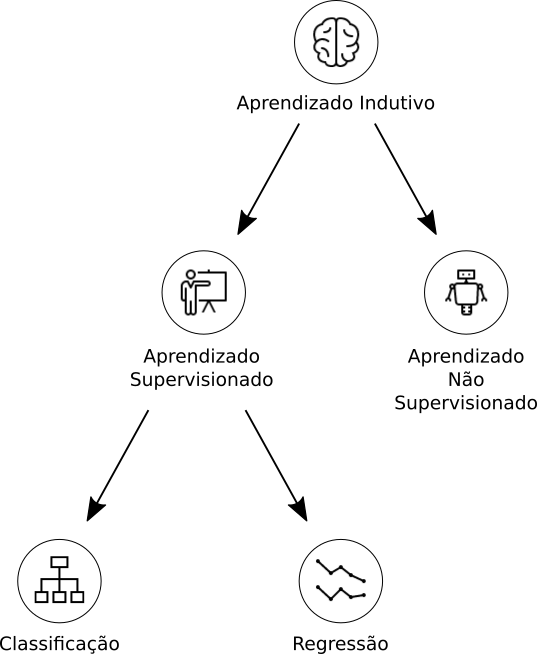
\includegraphics[scale=0.75]{figuras/aprendizado_indutivo.png}
\end{center}
\caption{A hierarquia do aprendizado indutivo}
\label{fig:aprendizado_indutivo}
\end{figure}

De acordo com ~\cite{porthos_motta:2016} classificadores são utilizados para a predição de classes de objetos e pode ser dita como o processo de generalização dos dados a partir de diferentes instâncias. Existe uma tendência de se referir a problemas com uma resposta quantitativas como problemas de regressão e aqueles com uma resposta qualitativa como problemas de classificação.

Dado um conjunto de exemplos como ilustrado na Figura ~\ref{fig:processo_classificacao}, os classificadores devem encontrar uma função geral capaz de prever adequadamente as saídas para novos exemplos, após o treinamento, o classificador é avaliado e se necessário o processo de classificação pode ser ajustado usando o conhecimento sobre o domínio do problema para escolher os dados de entrada ao algoritmo de aprendizado. 

% processo de classificação

\begin{figure}[H]
\begin{center}
    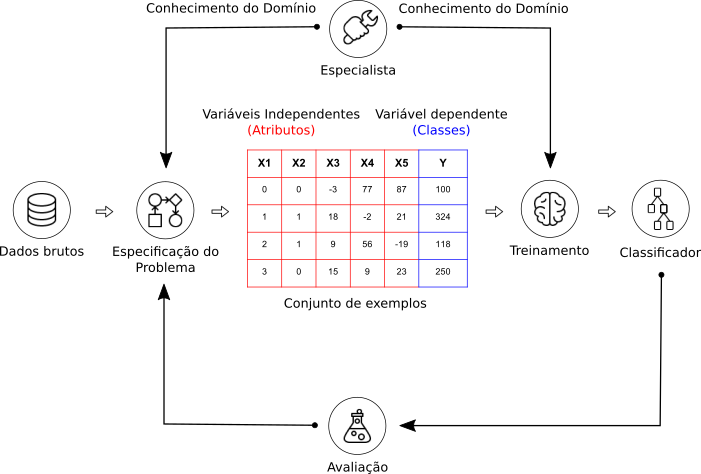
\includegraphics[scale=0.75]{figuras/processo_classificacao.png}
\end{center}
\caption{Processo de Classificação}
\label{fig:processo_classificacao}
\end{figure}

% 4) Orange mineração de dados

\section{Ferramenta para mineração de dados}

Diversas ferramentas disponíveis para exploração de dados dispõem de soluções para o processamento e a análise das informações de forma agil e simples. Em uma analise comparativa ~\cite{boscarioli2014avaliaccao} demonstra que não existe uma única ferramenta com caracteristicas melhores para todas as aplicações em mineração de dados.

Em um estudo que comparou quatro ferramentas (KMINE, \textit{Orange}, Tanagra, Weka), todas de código aberto, gratuitas e muito utilizadas na pesquisa e na academia, ~\cite{wahbeh2011comparison} concluiu que a ferramenta Weka apresentou o melhor desempenho, seguido pelo \textit{Orange}, e, depois, pelo KMINE e Tanagra.

Para este trabalho, foi escolhida a ferramenta \textit{Orange} ~\cite{JMLR:demsar13a} por ser muito utilizada no meio acadêmico, ter sido bem avaliada quando comparada a outras, ser utilizada como uma biblioteca na linguagem Python ~\cite{van2003python} e utiliza a conceituada biblioteca \textit{Scikit-learn} ~\cite{scikit-learn} internamente para aprendizado de máquina. 

A ferramenta \textit{Orange} na atual versão 3.4 desenvolvida pelo laboratório de Inteligência Artificial da Faculdade de Computação e Ciência da Informação da Universidade de Ljubljana na Eslovênia sob a licença GPL, possui uma interface gráfica denominada \textit{Orange Canvas}. Por meio de sua interface ilustrada na Figura ~\ref{fig:orange_canvas} é possível conectar e interligar os objetos montando um fluxo de trabalho para o desenvolvimento de modelos de classificação, incluindo Adaboost, Naive Bayes, Regras de Decisão, Árvores de Decisão, etc..

\begin{figure}[H]
\begin{center}
    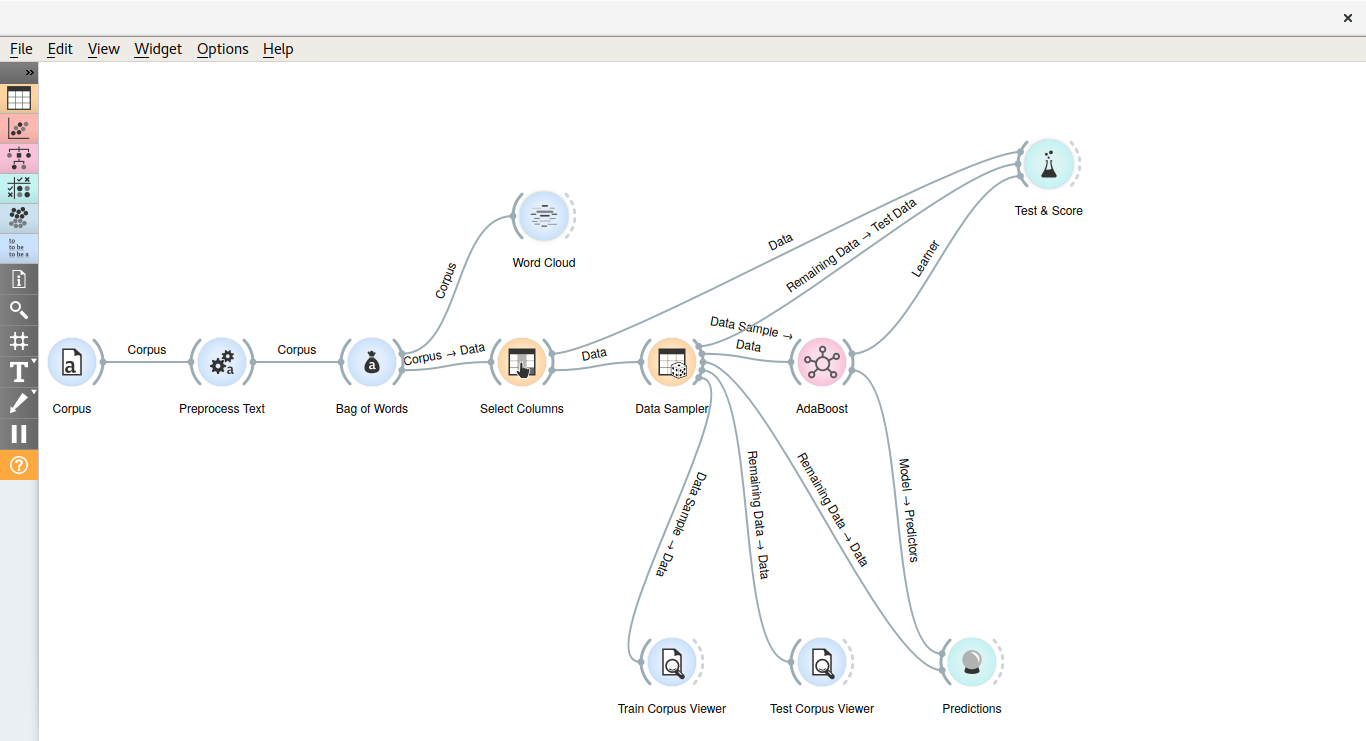
\includegraphics[scale=0.30]{figuras/orange_canvas.png}
\end{center}
\caption{Interface gráfica \textit{Orange Canvas}}
\label{fig:orange_canvas}
\end{figure}

% Este objetivo foi relevante para nosso estudo porque sabemos que as condições de

\chapter{Fundamentação Teórica}\label{fund_teo}

\section{Processamento de linguagem natural}
% Como explicado na secção anterior, existem diversas técnicas de processamento de linguagem natural, umas mais específicas e outras mais genéricas. Neste projecto foram implementados dois processos considerados relevantes, tokenization e o POS Tagger (Part of Speech Tagger). O processo de tokenization realiza a divisão do texto em tokens, de modo a facilitar o tratamento posterior de cada token de forma independente. Para a realização desta operação é necessário importar os modelos treinados da ferramenta OpenNLP, que contêm as regras necessárias para a correcta execução dos diversos métodos de processamento.

% Também é determinada a classe gramatical de cada componente das frases analisadas (POS Tagger), sendo necessária a importação do modelo treinado do OpenNLP para uma correta avaliação. Desta forma é possível identificar elementos importantes na frase, como os substantivos e adjectivos, para posteriormente estabelecer a correta polaridade da frase. Segue-se um exemplo5 do resultado deste processo aplicado à uma mensagem específica:

\section{Tokenizer}
\section{Bag of words}
\section{Aprendizado de máquina}
\section{Adaboost}
\section{Naive Bayes}
\section{Testes Scores}

\chapter{Método Proposto}\label{meto}

Para concluir com êxito o desenvolvimento deste trabalho e consequentemente os objetivos propostos, o método utilizado para solução do problema é composto das seguintes etapas sequenciais:

Como já foi dito o banco de redações UOL foi desenvolvido e armazenado em páginas HTML, o que permite o uso de um \textit{Web Crawler}, um algoritmo que explora a estrutura de grafo da \textit{Web} para navegar de uma página para outra. A Figura ~\ref{fig:metodologia_1} ilustra a etapa que o\textit{Web Crawler} recupera as páginas, filtra as redações avaliadas e coleta cada uma para um repositório local.

\begin{figure}[H]
\begin{center}
    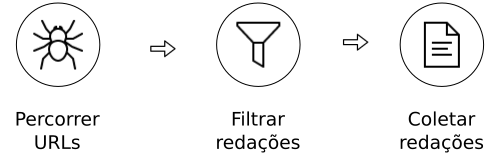
\includegraphics[scale=0.75]{figuras/metodologia_1.png}
\end{center}
\caption{Um \textit{Web Crawler}, navega entre as páginas HTML do banco de redações UOL de forma metódica e automatizada indexando textos de redações que posteriormente serão filtrados e coletados.}
\label{fig:metodologia_1}
\end{figure}

Na etapa subsequente a Figura ~\ref{fig:metodologia_2} ilustra a normalização dos textos, que consiste em uma técnica de remoção de caracteres não alfa-numéricos presentes no HTML e espaços desnecessários, tal que o valor textual ainda seja o mesmo que o original. Após a normalização será organizado as as diversas partes que compõem a redação (tema, título, texto e nota) em uma estrutura JSON para armazenamento e uso futuro. 

\begin{figure}[H]
\begin{center}
    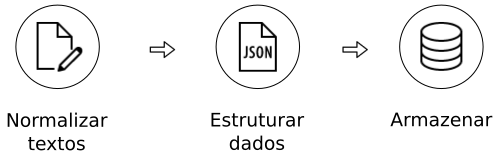
\includegraphics[scale=0.75]{figuras/metodologia_2.png}
\end{center}
\caption{Os textos são submetidos aos algoritmos de normalização e posteriormente estruturados e armazenados no padrão JSON.}
\label{fig:metodologia_2}
\end{figure}

Na terceira etapa ilustrada pela Figura ~\ref{fig:metodologia_3} será utilizada a ferramenta de mineração de dados \textit{Orange} ~\cite{JMLR:demsar13a}. Será necessário realizar estudo e análise para obter o conhecimento necessário para desenvolvimento de um fluxo de trabalho, seleção e treinamento dos modelos classificadores, concluindo todos os objetivos propostos nesta etapa.

\begin{figure}[H]
\begin{center}
    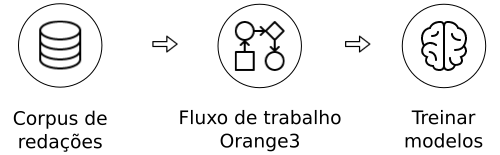
\includegraphics[scale=0.75]{figuras/metodologia_3.png}
\end{center}
\caption{O \textit{corpus} será utilizado em um fluxo de trabalho da ferramenta \textit{Orange} para treinar os modelos classificadores.}
\label{fig:metodologia_3}
\end{figure}

A quarta e última etapa é ilustrada pela Figura ~\ref{fig:metodologia_4}, onde os modelos classificadores previamente ajustados e treinados serão submetidos aos testes de Acurácia (taxa de predições corretas ou incorretas realizada pelo modelo para um determinado conjunto de dados), \textit{Overfitting} (super-ajustamento que ocorre quando o modelo se especializa nos dados utilizados no seu treinamento) e \textit{Noise} (\textit{noise} ou ruido é classificação errada do conjunto de dados de entrada), os resultados serão representados e comparados graficamente.
\begin{figure}[H]
\begin{center}
    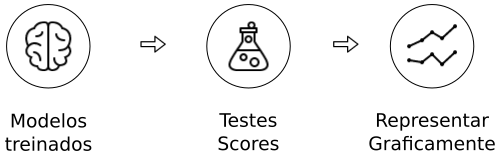
\includegraphics[scale=0.75]{figuras/metodologia_4.png}
\end{center}
\caption{O modelos ajustados e treinados serão submetidos a testes, e os resultados comparados graficamente.}
\label{fig:metodologia_4}
\end{figure}

\chapter{Desenvolvimento}\label{desen}

\chapter{Resultados Preliminares}\label{result}

Este capítulo é dedicado a apresentar os resultados preliminares e adversidades obtidas na indução do classificador \textit{AdaBoost}, um algoritmo que utiliza \textit{Boosting} como método de aprendizagem, flexível para se combinar com os vários algoritmos base de aprendizagem disponíveis.

\section{Dados Desbalanceados}

Para a indução do classificador AdaBoost sobre a primeira competência exigida em um texto de redação, isto é,  ``Demonstrar domínio da norma padrão da língua escrita.'', a ferramenta \textit{Orange} selecionou de forma aleatória uma amostra de 30\% do corpus de redações, ou seja, aproximadamente 131 redações de 436. 

A qualidade dos dados no \textit{dataset} é uma fator fundamental neste processo de indução, e trabalhar com dados desbalanceados tende à produzir regras de classificação que beneficiam as classes majoritárias, isto é, com maior probabilidade de ocorrência, resultando em uma baixa taxa de predição para o grupo minoritário.

Como demostrado no Gráfico ~\ref{gra:class_unbundling}, a amostra de 30\% das redações selecionadas no \textit{dataset} apresentou dados desbalanceados, ou seja, 70\% da amostra selecionada tende para as classes 0.50 e 1.00, os demais 30\% restante, para as classes 0.00, 1.50 e 2.00. 

\pgfplotstableread[row sep=\\,col sep=&]{
    class & score  \\
    0.00  & 15 \\
    0.50  & 40 \\
    1.00  & 52 \\
    1.50  & 20 \\
    2.00  & 4  \\
    }\mydata

\begin{figure}[H]
\begin{center}
\begin{tikzpicture}
    \begin{axis}[
            ybar,
            width=8cm,
            height=7cm,
            symbolic x coords={0.00,0.50,1.00,1.50,2.00},
            bar width=10pt,
            ylabel=Quantidade,
            xlabel=Classes,
            xtick=data,
            axis lines*=left,
        ]
        \addplot[draw=black, fill=white] table[x=class,y=score]{\mydata};
        \node [above] at (axis cs:  0.00,15) {15};
        \node [above] at (axis cs:  0.50,40) {40};
        \node [above] at (axis cs:  1.00,52) {52};
        \node [above] at (axis cs:  1.50,20) {20};
        \node [above] at (axis cs:  2.00,4) {4};
    \end{axis}
\end{tikzpicture}
\caption{Distribuição das classes em uma amostra de 131 redações selecionadas aleatoriamente no \textit{dataset}.}
\label{gra:class_unbundling}
\end{center}
\end{figure}

O desbalanceamento de dados presente na amostra era uma condição esperada, no processo de valoração, a competência é avaliada por, pelo menos, dois avaliadores, de forma independente, se ocorrer diferenças nas notas da competência inferior a 20\% entre elas, é calculado o valor médio, fator que colabora efetivamente para tendência de uma ou mais classes presentes na amostra.

\section{Métricas de Desempenho}

Nos resultados preliminares, este estudo utilizou as principais métricas da literatura para análise do desempenho de classificadores, tendo como foco as métricas: Curva ROC, Acurácia, \textit{F-Score}, \textit{Precision} e \textit{Recall}.

A Tabela ~\ref{tab:evaluation_result} exibe os resultados das principais métricas de desempenho de classificadores sobre cada classe induzida e também a média geral de cada métrica.

\begin{table}[H]
\centering
\begin{tabular}{c|c|c|c|c|c|}
\cline{2-6}
 & \multicolumn{5}{c|}{\textbf{Resultado da avaliação}} \\ \hline
\multicolumn{1}{|c|}{\textbf{Classes}} & \textbf{ROC} & \textbf{Acurácia} & \textit{\textbf{F-Score}} & \textit{\textbf{Precision}} & \textit{\textbf{Recall}} \\ \hline
\multicolumn{1}{|c|}{\textbf{0.00}}  & 0.498 & 0.828 & 0.096 & 0.845 & 0.828 \\ \hline
\multicolumn{1}{|c|}{\textbf{0.50}}  & 0.552 & 0.640 & 0.349 & 0.653 & 0.640 \\ \hline
\multicolumn{1}{|c|}{\textbf{1.00}}  & 0.499 & 0.509 & 0.422 & 0.506 & 0.509 \\ \hline
\multicolumn{1}{|c|}{\textbf{1.50}}  & 0.549 & 0.579 & 0.222 & 0.755 & 0.759 \\ \hline
\multicolumn{1}{|c|}{\textbf{2.00}}  & 0.541 & 0.915 & 0.140 & 0.899 & 0.915 \\ \hline
\multicolumn{1}{|c|}{\textbf{Média}} & \textbf{0.529} & \textbf{0.694} & \textbf{0.246} & \textbf{0.737} & \textbf{0.730} \\ \hline
\end{tabular}
\caption{Resultado das métricas de desempenho do classificador AdaBoost.}
\label{tab:evaluation_result}
\end{table}

A adversidade de classes desbalanceadas, pode produzir um modelo com elevadas taxas de acurácia global para determinadas classes, como o ocorrido nas classes 0.00 e 2.00 de 0.828 e 0.915 respectivamente, entretanto frequentemente tende a prejudicar a identificação de exemplos pertencentes a grupos minoritários.

Ilustrada na Figura ~\ref{fig:roc}, a representação gráfica da Curva ROC de cada classe induzida pelo classificador.

\begin{figure}[H]
\begin{center}
    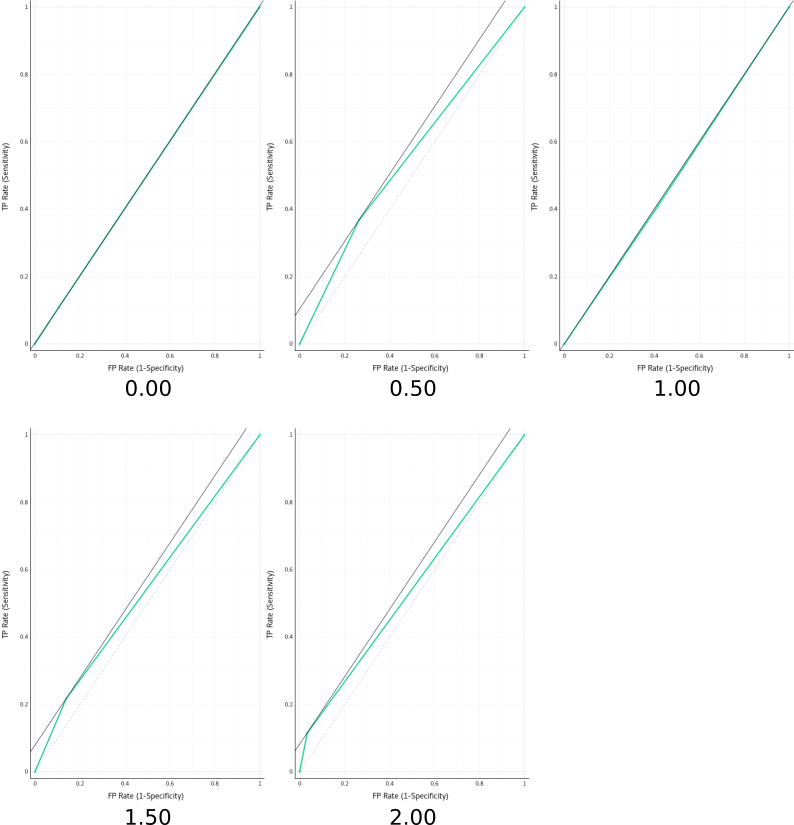
\includegraphics[scale=0.75]{figuras/roc.png}
\end{center}
\caption{Representação gráfica da Curva ROC para cada classe (0.00, 0.50, 1.00, 1.50 e 2.00) induzida no modelo AdaBoost.}
\label{fig:roc}
\end{figure}

O comportamento esperado para a curva, é que a mesma, se aproxime o máximo possível de 1 em cada classe. Entretanto a métrica se apresenta como uma reta nas classes 0.00 e 1.00, nas demais classes tende sutilmente a 1. Conclui-se que a predição das classes 0.00 e 1.00 nos testes estão ocorrendo de forma aleatório pelo classificador.

Por fim a tabela de contingência ou matriz de confusão, que através da discriminação dos erros ou acertos preditos para cada classe demonstra o desempenho do classificador, uma das métricas mais eficiente de se analisar um classificador. 

A Tabela ~\ref{tab:matrix_confusion} exibe ao longo da diagonal em tons de cinza as decisões corretas: número de verdadeiros positivos TP e verdadeiros negativos TN; já os elementos fora dessa diagonal representam os erros cometidos: número de falsos positivos FP e falsos negativos FN. É notável que o valor ideal fora da diagonal seja sempre igual a 0.  

\begin{table}[H]
\centering
\begin{tabular}{cc|c|c|c|c|c|c|}
\cline{3-8}
 &  & \multicolumn{6}{c|}{\textbf{Predição}} \\ \cline{3-8} 
 &  & \textbf{0.00} & \textbf{0.50} & \textbf{1.00} & \textbf{1.50} & \textbf{2.00} & $\sum_{}$  \\ \hline
\multicolumn{1}{|c|}{} & \textbf{0.00} & \cellcolor[HTML]{C0C0C0}4 & 18 & 13 & 2 & 0 & \textbf{37} \\ \cline{2-8} 
\multicolumn{1}{|c|}{} & \textbf{0.50} & 13 & \cellcolor[HTML]{C0C0C0}42 & 44 & 14 & 1 & \textbf{114} \\ \cline{2-8} 
\multicolumn{1}{|c|}{} & \textbf{1.00} & 18 & 51 & \cellcolor[HTML]{C0C0C0}78 & 32 & 11 & \textbf{190} \\ \cline{2-8} 
\multicolumn{1}{|c|}{} & \textbf{1.50} & 7 & 14 & 31 & \cellcolor[HTML]{C0C0C0}15 & 2 & \textbf{69} \\ \cline{2-8} 
\multicolumn{1}{|c|}{} & \textbf{2.00} & 4 & 2 & 14 & 3 & \cellcolor[HTML]{C0C0C0}3 & \textbf{26} \\ \cline{2-8} 
\multicolumn{1}{|c|}{\multirow{-6}{*}{\rot{Atual}}} & $\sum_{}$ & \textbf{46} & \textbf{127} & \textbf{180} & \textbf{66} & \textbf{17} & \textbf{436} \\ \hline
\end{tabular}
\caption{Tabela de contingência ou Matriz de confusão resultante da indução do classificador AdaBoost.}
\label{tab:matrix_confusion}
\end{table}

\section{Considerações Finais}

E notável que adversidade de classes desbalanceadas influenciou consideravelmente nos resultados preliminares.  A próxima etapa deste estudo merece destaque em uma seção exclusiva para discussão do tema e a análise dos principais métodos na literatura para balanceamento de classes.

As dificuldades observadas no estudo do problema proposto motivam melhorias e o surgimento de novas estratégias pra a continuidade do trabalho. 

% Os primeiros experimentos realizados na predição, ilustrado no Gráfico abaixo, demonstraram uma taxa de 30\% de acerto na predição da primeira competência exigida em um texto de redação, de uma amostra de 100 redações. 

% A análise gráfica do resultado experimental demonstra que a predição do modelo está em uma faixa especifica de 0.5 a 1.5, ou seja, a indução do modelo deve ser repetida até o mesmo se tornar genérico.

% \pgfplotstableread[col sep=semicolon]{data/adaboost_competence_1.dat}\data
% \begin{figure}[H]
% \begin{center}

% \begin{tikzpicture}
%     \begin{axis}[
%         title=Demonstrar domínio da norma padrão da língua escrita. (1ªCompetência ),
%         width=\textwidth,
%         ymin=0,
%         ytick={0,0.5,1.0,1.5,2.0},
%         ylabel=Pontuação,
%         xtick=data,
%         xticklabel style={rotate=90,anchor=east},
%         xticklabels from table={\data}{title},
%         legend style={ legend columns=-1},
%         enlarge x limits=0.01
%         ]
%         \addplot table[x=id, y=comp1] {\data};
%         \addplot table[x=id, y=adaboost] {\data};
%         \legend{Profissional,AdaBoost}
%     \end{axis}
% \end{tikzpicture}
% \end{center}
% \end{figure}


\chapter{Conclusão e Trabalhos Futuros}\label{conc}



%%%% Estilo de citação ABNT e arquivo de bibitens (bib.bib)
\bibliographystyle{configuracao/abnt-alf}
\bibliography{bibliografia/bib}

\apendice
\chapter{Título do Apêndice}
\label{Apx:A}




\chapter{Exemplo do pacote Algorithm}
\label{Apx:B}


\begin{algorithm}[!h]
\caption{Estimador ML otimizado.}\label{Alg:MAXVER}
\begin{algorithmic}[1]
\STATE Inicializar o contador: $j\leftarrow 1$;%
\STATE Fixar o limiar de variação das estimativas: $e_{\mathrm{out}}\leftarrow 10^{-4}$;%
\STATE Fixar o número máximo de iterações: $N\leftarrow 1000$;%
\STATE Computar o ponto inicial: $\hat \gamma(0)$;%
\STATE Determinar o limiar inicial: $e_1 \leftarrow1000$;%
\STATE Estabelecer o valor inicial de $\alpha$: $\hat \alpha(0) \leftarrow -10^{-6}$;%
\WHILE{ $e_j \geq e_{\mathrm{out}}$ e $ j\leq M$}
    \STATE Solucionar $\hat \alpha_j\leftarrow {\arg \max}_{\alpha}\;{l_1(\alpha; \gamma_{j-1},\mathbf{z},n)}$;%
    \STATE Solucionar $\hat \gamma_j\leftarrow {\arg \max}_{\gamma}\;{l_2(\gamma; \alpha_j,\mathbf{z},n)}$;%
    \STATE $j\leftarrow j+1$
    \STATE Computar o critério de convergência: $e_j$;%
\ENDWHILE
\end{algorithmic}
\end{algorithm}


\end{document}